\section{Physical Fundamentals}
\subsection{Electronic Transport}
\subsubsection{Drude Model}
\begin{itemize}
  \item Electric field applied to conducting material accelerates carriers
  \item Carriers are scattered by impurities and lattice atoms
        \begin{align*}
          &\vec{v}_{D} = \mu \vec{E} &\text{: mean drift velocity},\\
          &\vec{j} = en\vec{v}_{D} &\text{: elec. current density},\\
          \implies&\vec{j} = \underbrace{en\mu}_{\sigma} \vec{E} = \sigma_{n} \vec{E}
        \end{align*}
  \item Two carrier species in semiconducting materials: electrons and holes
  \item Driving force of drift current is electric potential $\varphi$
        \begin{align*}
          &\vec{j_{n}}(\vec{r}) = en\mu_{n}\vec{E} = \sigma_{n}\vec{E} = -\sigma_{n}\nabla\varphi,\\
          &\vec{j_{p}}(\vec{r}) = en\mu_{p}\vec{E} = \sigma_{p}\vec{E} = -\sigma_{p}\nabla\varphi
        \end{align*}
        \item Additional driving force in semiconductors is gradient of carrier concentration
        \begin{align*}
          &\vec{j}_{n}(\vec{r}) = eD_{n}\nabla n,\\
          &\vec{j}_{p}(\vec{r}) = eD_{p}\nabla p,\\
          &D_{n,p} = \dfrac{kT}{q}\mu_{n,p} & \text{: Einstein's relation}
        \end{align*}
  \item \textbf{Drift-diffusion} model for electrons and holes
        \begin{align*}
          &\vec{j}_{n}(\vec{r}) = en\mu_{n}\vec{E} + \mu_{n}kT\nabla n\\
          &\vec{j}_{p}(\vec{r}) = \underbrace{en\mu_{p}\vec{E}}_{\text{drift current}}
          + \underbrace{\mu_{p}kT\nabla p}_{\text{diffusion current}}
        \end{align*}
\end{itemize}

\subsubsection{Continuity Equations}
\begin{align*}
  \dfrac{\partial n}{\partial t} = \dfrac{1}{e} \mathrm{div}\,\vec{j}_{n}(\vec{r}) + G - R + \dfrac{\partial N_{D}^{+}}{\partial t}\\
  \dfrac{\partial p}{\partial t} = \dfrac{1}{e} \mathrm{div}\,\vec{j}_{p}(\vec{r}) + G - R + \dfrac{\partial N_{A}^{-}}{\partial t}\\
\end{align*}

\subsection{Structure of Matter}
\begin{itemize}
  \item Energie levels of free particals can be described by a parabols $E = f(p^{2}, k^{2})$ in $k$-space.
        \begin{equation*}
          E = \dfrac{p^{2}}{2m} = \dfrac{\hbar^{2}\cdot k^{2}}{2m}
        \end{equation*}
  \item Parabolic Approximation: locally at minima and maxima for energy bands
\end{itemize}

\begin{definition}{Density of States $N_{n,p}(E)$ (Zustandsdichte)}
  The number (or density) of states per energy intervall $\mathrm{d}E$. Useful for calculating the number of carriers $n$ or $p$.

  For parabolic bands:
  \begin{align*}
    N_{n}(E) \, \mathrm{d}E = \dfrac{2\pi \cdot {(2m_{n}^{*})}^{3/2}}{h^{3}} \sqrt{E - E_{c}} \, \mathrm{d}E\\
    N_{p}(E) \, \mathrm{d}E = \dfrac{2\pi \cdot {(2m_{p}^{*})}^{3/2}}{h^{3}} \sqrt{E_{v} - E} \, \mathrm{d}E\\
  \end{align*}
\end{definition}

\begin{itemize}
  \item Fermi-Dirac distribution describes electron (fermion) distribution
        \begin{equation*}
          f_{\mathrm{FD}}(E) = \dfrac{1}{1 + \exp \left(\dfrac{1}{kT} (E - E_{F})\right)}
        \end{equation*}
  \item For parabolic bands:
        \begin{equation*}
          f_{\mathrm{FD}}(E) \approx \exp \left(- \dfrac{E_{\mathrm{gap}}}{2 kT}\right)
        \end{equation*}
  \item $n(T)$ and $p(T)$ determined by integrating over the respective energy space:
        \begin{equation*}
        n(T) = \int N_{n}(E)f(T, E) \, \mathrm{d}E
        \end{equation*}
  \item Mass action law for carrier concentration (also for doped semiconducters)
        \begin{equation*}
          n_{i}^{2} = n \cdot p
        \end{equation*}
\end{itemize}

\subsection{Charateristic Properties of Semiconductors}
\begin{itemize}
  \item Electric conductivity depends on carrier number $n$ or $p$ and mobility $\mu$
        \begin{equation*}
          \sigma_{\alpha} = e\alpha \mu_{\alpha}, \quad \alpha = n, p
        \end{equation*}
  \item Carrier mobility:
        \begin{align*}
          \mu_{\alpha} := \dfrac{|\vec{v}_{\alpha}|}{|\vec{E}|} = e \dfrac{\tau_{\alpha}}{m_{\alpha}}, \quad \alpha = n, p, \quad [\mu] = \dfrac{\si{cm^{2}}}{\si{Vs}}
        \end{align*}
  \item Carrier mobility depends on
        \begin{itemize}
                \item Temperature $\mu \propto T^{\beta}$ with $\beta \approx \begin{cases}+3/2, \quad \text{for low T (impurity scattering)}\\ -3/2, \quad \text{for high T (phonon scattering)} \end{cases}$
                \item Doping concentration: scattering throught ionized impurities reduces $\tau_{\alpha}$
        \end{itemize}
        \begin{tabular}{cc}
          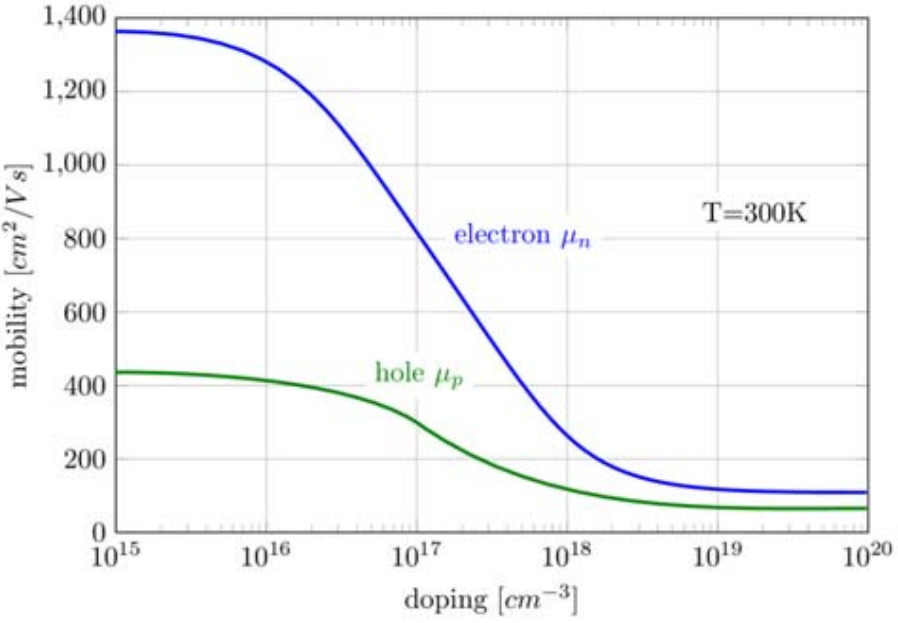
\includegraphics[width=.25\textwidth]{content/bdml/pictures/electron_vs_hole_mobility}
          &
          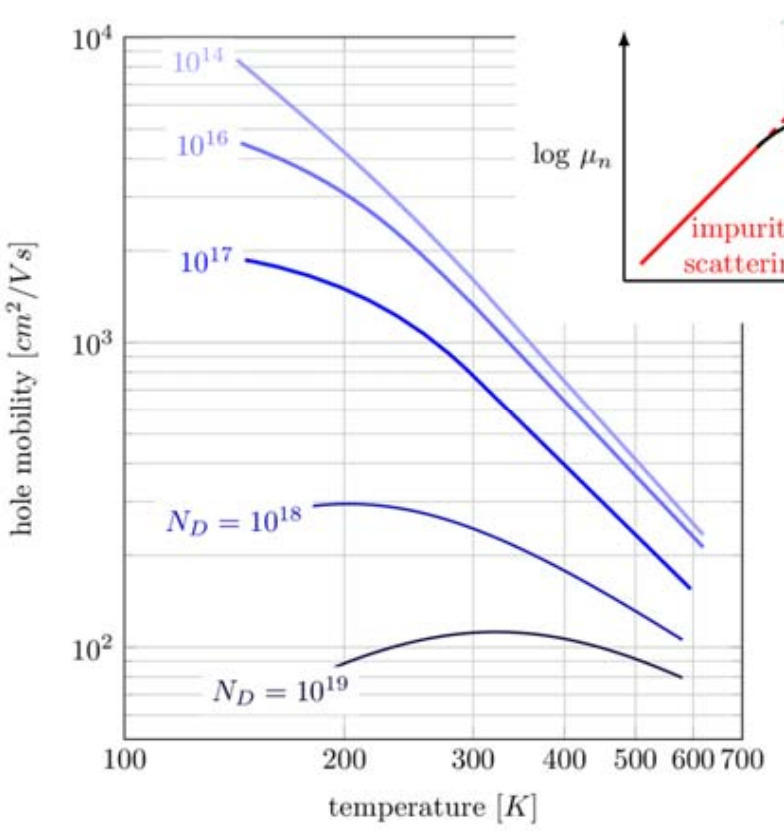
\includegraphics[width=.22\textwidth]{content/bdml/pictures/hole_mobility_doping}
        \end{tabular}
  \item Scattering of carriers:
        \begin{enumerate}
          \item impurity scattering (doping dependence)
          \item phonon scattering (temperature dependence)
          \item carrier-carrier scattering
        \end{enumerate}
        \item Drift velocity $\vec{v}_{D}$ saturates for high $\vec{E}$ $\implies$ $\lim\limits_{\vec{E} \to \infty} \vec{v}_{D} = const$
  \item Elec. conductivity
        \begin{equation*}
          \sigma = \dfrac{1}{\rho} = q \, (n\mu_{n} + p\mu_{p})
        \end{equation*}
  \item Thermal heat flow:
        \begin{equation*}
          \vec{J}_{Q} = -\kappa \, \nabla T
        \end{equation*}
  \item Elec. and thermal conductivity related by \textbf{Wiedenmann-Franz} law:
        \begin{equation*}
          \dfrac{\kappa_{n}}{\sigma_{n}} = L \, T, \quad L = \begin{cases} \dfrac{1}{3}{\left(\dfrac{\pi k_{B}}{e}\right)}^{2} \quad \text{metal}\\ 2{\left(\dfrac{k_{B}}{e}\right)}^{2} \quad \text{semiconducter} \end{cases}
        \end{equation*}
\end{itemize}
